\section{Control Module}

The control module is responsible for coordinating the activity of the
other parts of the image processor and for data transfer into and within
the image processor. A visual overview of the control module is given in
figure \ref{fig:control-module}.

\begin{figure}[h!]
\centering
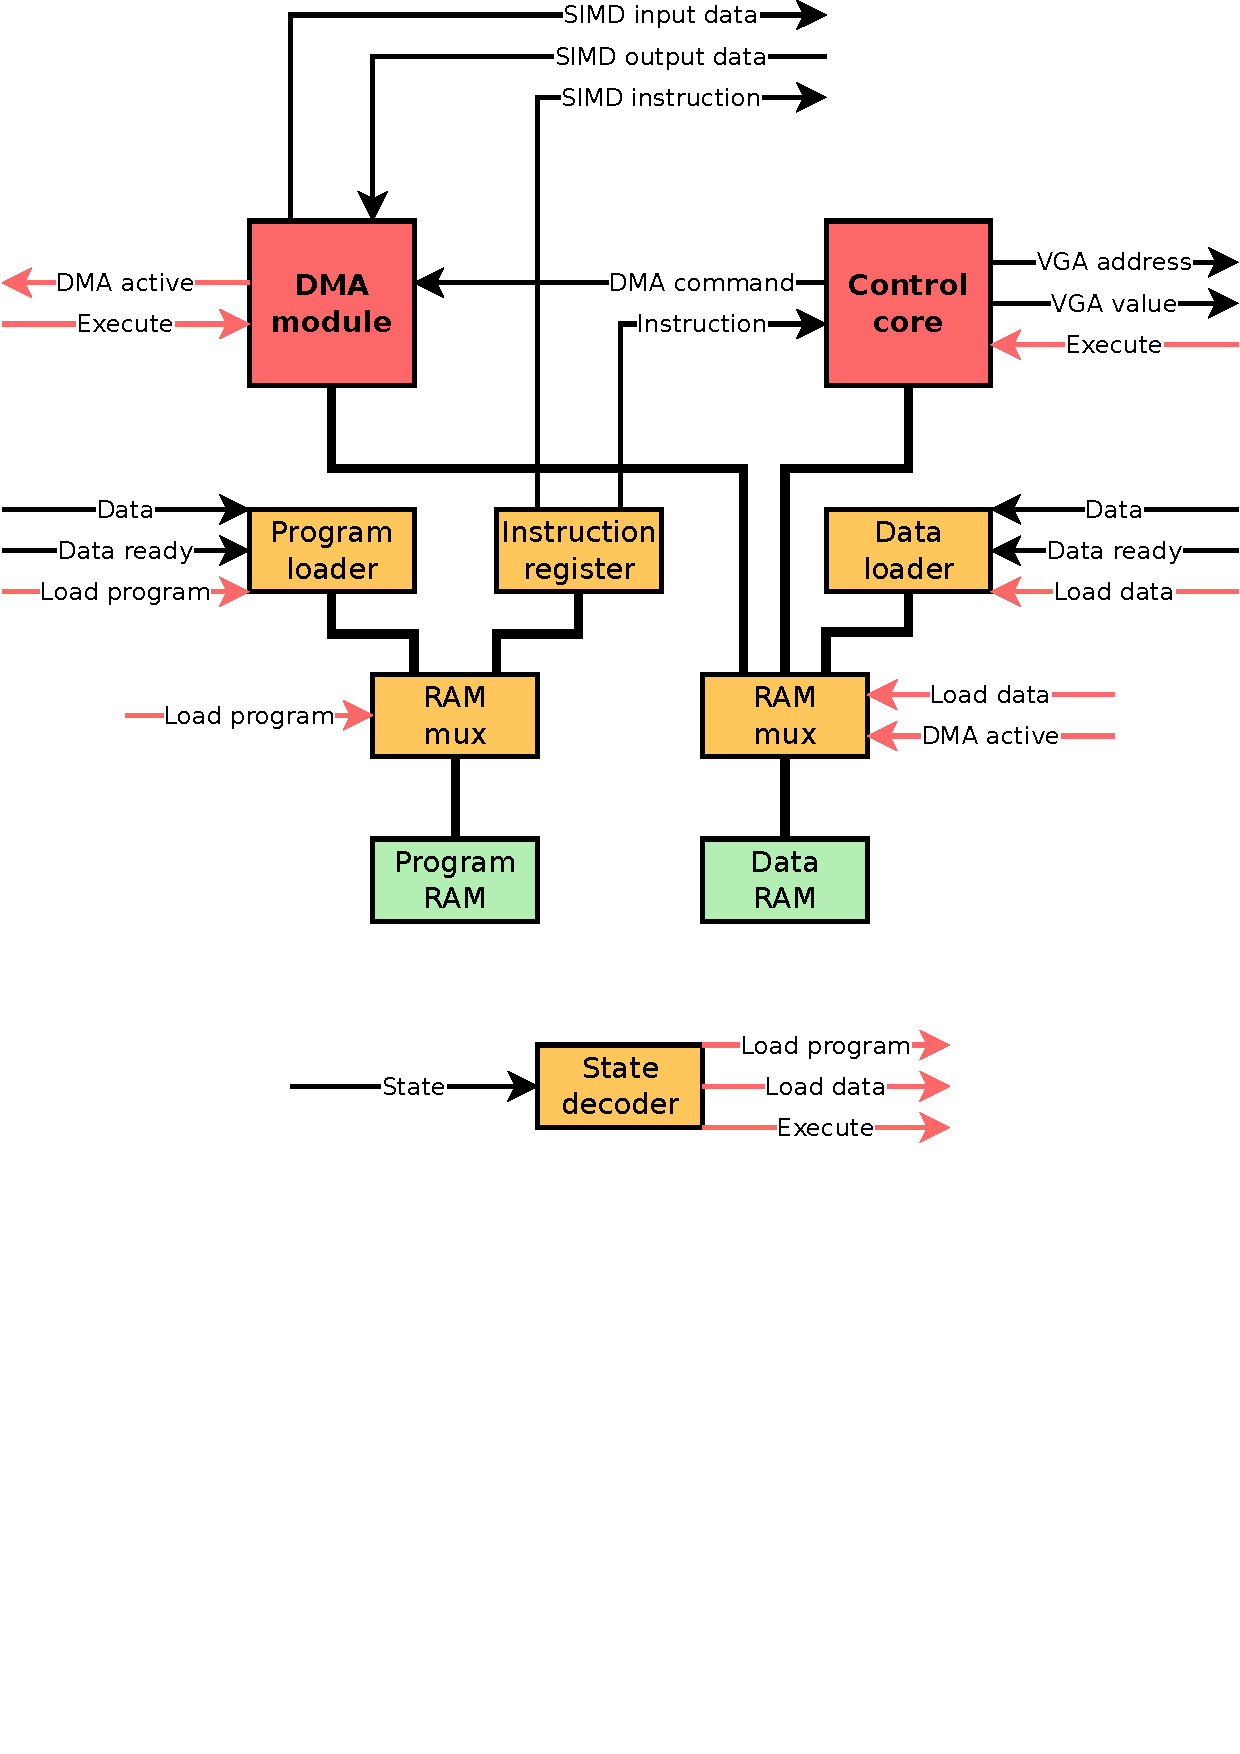
\includegraphics[width=\linewidth,clip,trim=0 10cm 0 0]
                {fig/fpga/control_module.pdf}
\caption[Control module]
        {An overview of the control module of the image processor.}
\label{fig:control-module}
\end{figure}


The control module decodes the state signal set by the AVR, and enables,
disables and resets components accordingly. It is responsible for
performing data transfers between the AVR and the program/data memories,
and for transferring data internally, between the SIMD node array, data
RAM and the VGA screen buffer.

The control module contains the CPU core that is used for the non-SIMD
instructions embedded in a program. This CPU core, henceforth referred
to as the \emph{control core}, is mainly concerned with loop control,
initiating data transfers between the SIMD node array and the data RAM,
and copying image data to the VGA controller.

\subsection{States}

The operation of the image processor is fully controlled by the SCU. The
SCU sets a state value that is used by the control module to select
which components of the image processor are active. This is indicated by
the red signals in figure \ref{fig:control-module}.

The states recognized by the image processor are listed in table
\ref{tab:states}.

\begin{table}[h]
  \centering
  \begin{tabular}{cl}\toprule
    \thx{State} & \thx{Description} \\ \midrule
    000 & Idle \\
    001 & Run program \\
    010 & Load data from SCU \\
    100 & Load program from SCU \\
    \bottomrule
  \end{tabular}
  \caption{Image processor states.}
  \label{tab:states}
\end{table}


\subsection{Control Core}

A schematic overview of the control core is given in figure
\ref{fig:fpga-ctrl-core}. The control core consists of a register bank
of 21 bit registers, an ALU and a connection to the data RAM. The word
width of 21 bits was chosen to match the address width of the data RAM.
This allows the control core to do pointer arithmetic referring to
arbitrary words in the data RAM.

\begin{figure}[h]
  \centering
  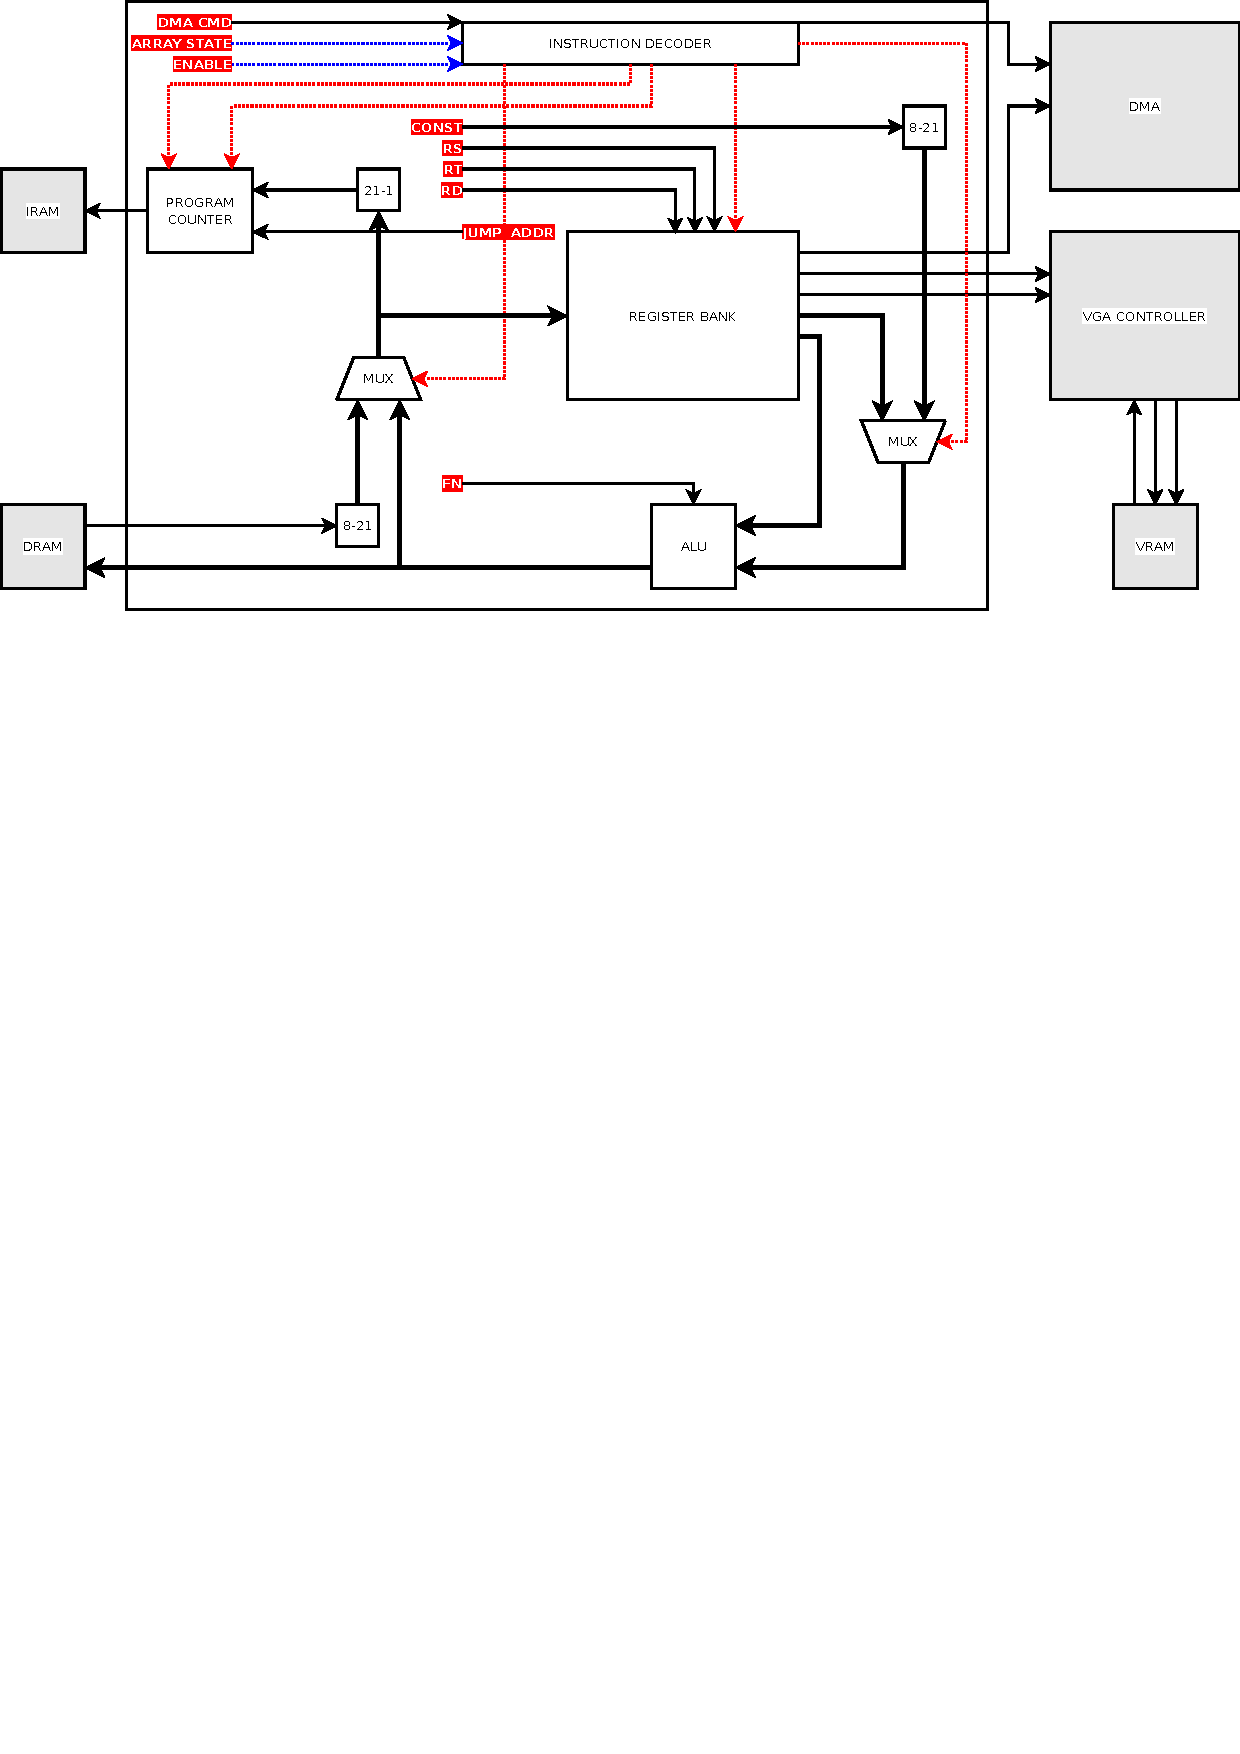
\includegraphics[width=\linewidth,clip,trim=0 18cm 0 0]
                  {fig/fpga/fpga_ctrl_core.pdf}
  \caption{Image processor control core.}
  \label{fig:fpga-ctrl-core}
\end{figure}


To send pixels to the VGA controller, two of the registers are dedicated
to contain an address and a pixel value, respectively. The contents of
these registers are constantly sent to the VGA controller. By
incrementing and loading RAM values into these registers, using the
control core's regular instruction set, the control core program can
upload images to the VGA screen buffer.

A third register is wired to the DMA controller, to enable 21 bit wide
DMA parameters to be set programmatically.

The control core runs instructions from the same instruction stream as
the SIMD nodes, and thus the control core and the SIMD array share a
common program counter. The leftmost bit in the instructions specifies
whether the instruction is a control core instruction or a SIMD
instruction.

The control core instruction set is specified in detail in appendix
\ref{app:control-inst}.

\subsection{DMA Module}

Because of the common instruction stream between the SIMD array and the
control core, the SIMD array will be inactive whenever the control core
is busy. An important task that normally would be the control core's
responsibility, is to load the SIMD array with new data from RAM and to
store the processed data back to RAM. To maximize the utilization of
the data RAM I/O capacity and the processing power of the SIMD array, a
\emph{Direct Memory Access module} was devised.

The DMA module performs loading of new SIMD data planes and storing of
processed SIMD data planes \emph{in parallell} with the normal execution
of program instructions. The nodes of the SIMD array have a separate
register -- the S register -- that is reserved for the DMA module. The S
registers are connected in a left-to-right direction throughout the
array. The DMA module can send the contents of the S registers one step
to the right by setting a \emph{step S} signal.

With these accommodations of the SIMD array, the DMA module can load new
data values to the S registers at the left edge of the SIMD array, send
the step signal to have these value propagate into the array and read
the old, processed data values from the S registers at the right edge of
the array. The SIMD program executing simultaneously will operate on a
different set of registers and will not be obstructed by the DMA data
transfer.

During DMA transfer, the data RAM is reserved for the DMA module and not
available for the control core to use. To initiate a DMA transfer, the
control core sets \emph{base addresses} for the reading of new data and
for the writing of old data, in addition to address increments to be
used for moving along the columns and rows of the current slice of the
data. These parameters allow flexibility in how the data slices to be
loaded into and stored out of the SIMD array, are laid out in memory.
